\documentclass[11pt,aspectratio=1610]{beamer}
\usepackage{fbb}
\usetheme{CambridgeUS}
\beamertemplatenavigationsymbolsempty
\usepackage[utf8]{inputenc}
\usepackage{amsmath,adjustbox,mathtools}
\usepackage{amsfonts}
\usepackage{hyperref}
\usepackage{graphicx}
\usepackage{xpatch}
\usepackage{makecell}
\usepackage{tabularx}
\usepackage{csquotes}
\usepackage{adjustbox}
\setbeamertemplate{caption}{\raggedright\insertcaption\par}
\usepackage{minted}
\usetheme{default}
\usecolortheme{default}


% Définition des couleurs
\definecolor{schTag}{RGB}{204, 0, 0}       % Rouge pour les balises
\definecolor{schAttr}{RGB}{0, 0, 153}      % Bleu pour les attributs
\definecolor{schValue}{RGB}{0, 102, 0}     % Vert pour les valeurs
\definecolor{schBg}{RGB}{245, 245, 245}    % Fond gris clair

% Configuration de minted
\setminted{
  bgcolor=schBg,
  frame=single,
  framesep=2mm,
  linenos=true,
  breaklines=true,
  fontsize=\small,
}


\usepackage{pgfplots}
\usepackage{tikz}
\usetikzlibrary{shapes,calc,matrix,decorations.markings,decorations.pathreplacing,positioning, intersections,backgrounds,through,hobby}
\usepackage[english]{babel}
%\AtBeginSection[]
%{\begin{frame}
% \frametitle{}  
%\setlength{\itemsep}{.5cm}
% \tableofcontents[currentsection,
%                  hideothersections,
%		  sectionstyle=hide/hide/hide,
%                  subsectionstyle=show/show/show/hide
%                   ]
% \end{frame} 
% }

%\AtBeginsection[]
%{\begin{frame}
% \frametitle{}  
% \tableofcontents[currentsection,
%	 	  currentsection,
%		  sectionstyle=show/hide,
%                  sectionstyle=show/shaded/hide
%                   ]
% \end{frame} 
% }


\AtBeginSection[]
{
  \begin{frame}
    \tableofcontents[
      currentsection,       % Met en évidence la section courante
      sectionstyle=show/shaded, % Sections : courante en évidence, autres en grisé
      subsectionstyle=hide  % Cache toutes les sous-sections
    ]
  \end{frame}
}
 
 

\AtBeginSubsection[]
{
  \begin{frame}
    \tableofcontents[
     currentsection, % Affiche uniquement la section courante
      hideothersubsections, % Cache les sous-sections des autres sections
      sectionstyle=show/hide, % Cache les autres sections
      subsectionstyle=show/shaded/hide % Sous-section courante en évidence, les autres en grisé
    ]
  \end{frame}
}


\setbeamertemplate{sections/subsections in toc}[square]
\setbeamertemplate{bibliography item}[sqare]
\setbeamertemplate{itemize item}[square]
\setbeamertemplate{enumerate item}[square]
\setbeamertemplate{itemize subitem}[square]




\setbeamertemplate{sections/sections in toc}[square]
\setbeamertemplate{itemize item}[square]
\setbeamertemplate{enumerate item}[square]
\setbeamertemplate{itemize subitem}[square]

\usepackage[style=verbose,citestyle=authoryear,isbn=true,url=false,
doi=true,backend=biber,maxbibnames=9, maxcitenames=4]{biblatex}
\addbibresource{/home/mgl/Bureau/Travail/Communications_et_articles/bibliographie_commune/biblio.bib}
\renewcommand*{\bibfont}{\tiny} 

\usepackage{tikz}
\usetikzlibrary{shapes,calc,matrix,decorations.markings,decorations.pathreplacing,positioning, intersections,backgrounds}
\tikzstyle{bag} = [align=center]

\date[24 mars 2026]{24 mars 2026}
\author[Matthias \textsc{Gille Levenson}]{\\~\\ Matthias \textsc{Gille Levenson}\\   {\scriptsize Université Versailles Saint Quentin (UVSQ) \& École Normale Supérieure de Lyon, France}\\ {\tiny matthias [dot] gille [-] levenson [at] ens-lyon [dot] fr}\vspace{-1cm}}
\title[Le XML]{Session 1: Introduction générale au XML\\ {\small Atelier Humanités Numériques \\ Lyon}}
%\titlegraphic{\hspace{0.5cm}\includegraphics[scale=0.21]{/home/mgl/Bureau/Travail/admin/logos/ensl.png}\hspace{0.5cm}\includegraphics[scale=0.23]{/home/mgl/Bureau/Travail/admin/logos/ciham.pdf}\hspace{0.5cm}}
\usepackage[justification=centering]{caption}
\begin{document}
\maketitle

\section{Introduction}


\begin{frame}{Accès aux slides}
\begin{itemize}
\item \href{https://github.com/matgille/formation_TEI_AHN_mars_2026.git}{https://github.com/matgille/formation\_TEI\_AHN\_mars\_2026.git}
\end{itemize}
\end{frame}

\section{Le format XML}
\subsection{Qu'est-ce que le XML?}

\begin{frame}{eXtensible Marking Language}
\begin{itemize}
\item XML signifie \textbf{eXtensible Markup Language}.
\item Il s'agit d'un format qui permet de décrire tout type de données textuelles (ou numériques) 
\item Il s'agit du \textit{format} actuellement utilisé par le TEI, mais il est susceptible de changer ou d'évoluer à l'avenir.
\end{itemize}
\end{frame}

\begin{frame}{Composants principaux du XML}
\begin{itemize}
\item Le XML peut être décomposés en éléments principaux, qu'on appelle des \textbf{noeuds}
\item Les noeuds principaux sont: le texte, les éléments, les attributs, les commentaires.
\item Ces noeuds sont représentés à l'aide de caractères spécifiques
\end{itemize}
\end{frame}


\begin{frame}{Vocabulaire}
Quatre objets principaux (appelés \textit{n\oe uds}) :
\begin{itemize}
\item N\oe uds \textbf{éléments} : l'objet de base de tout document XML : \\ \texttt{<elementName/>} ou \texttt{<elementName>...</elementName>}
\item N\oe uds \textbf{attributs} : partie d'un élément qui permet de le définir : \\ \texttt{attributeName="value"}
\item N\oe uds \textbf{texte} : tout objet textuel contenu dans un élément
\item N\oe uds \textbf{Commentaire} : contenu non traité par la machine : \\ \texttt{<!-{}- un commentaire utile -{}->}
\end{itemize}
\end{frame}

\subsection{Conformité et validité}
\begin{frame}{Conformité et validité}
\begin{itemize}
\item Un document \textbf{doit} être conforme au XML, c'est-à-dire respecter l'ensemble des règles du XML
\item Un document \textbf{peut} être validé par un \textbf{schéma}, c'est-à-dire un document qui vérifie des règles propres à une spécification particulière
\item Quelques spécifications XML: TEI, EAD, DublinCore, AltoXML, PageXML, RDF, etc...
%\item Along with validity comes another important concept/nightmare: \textit{namespaces}. You'll understand soon enough.
\item Nous nous intéresserons à la validité des documents XML dans la seconde session de la formation.
\end{itemize}
\end{frame}


\begin{frame}{Conformité. Composants principaux du XML}
\begin{itemize}
\item Il existe peu de règles en XML mais elles sont fondamentales:
\item Du point de vue de la \textit{modélisation} (représentation abstraite de l'objet XML)
\begin{itemize}
\item Règle d'enchâssement des éléments
\item Règle d'unicité des attributs
\end{itemize}
\item Du point de vue de la \textit{sérialisation} (expression de l'objet XML à l'aide d'une chaîne de caractères)
\begin{itemize}
\item Règles d'expression d'un élément
\item Règle d'expression des attributs: espaces et guillemets obligatoires
\end{itemize}
\end{itemize}
\end{frame}


\begin{frame}{Conformité. Composants principaux du XML}
\begin{center}
\begin{figure}
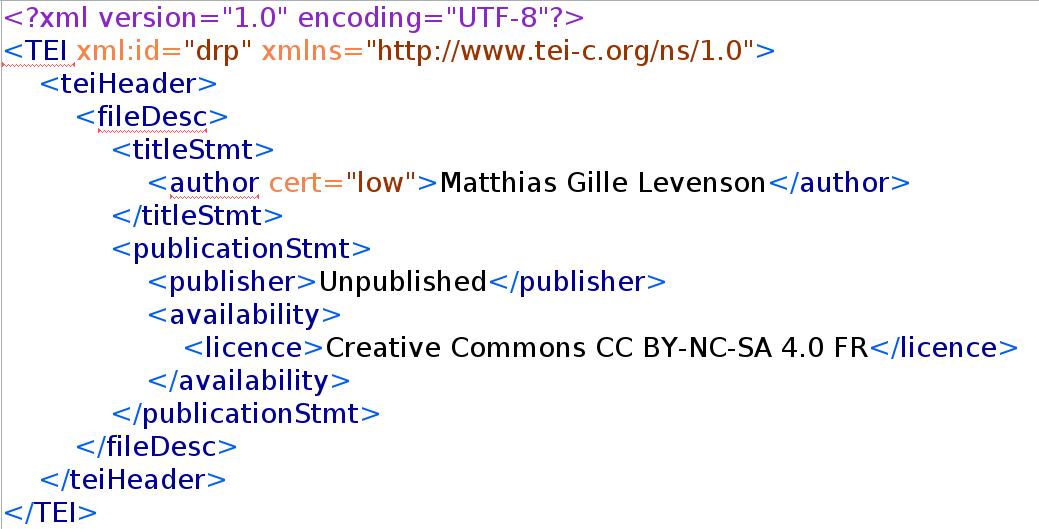
\includegraphics[height=.5\textheight]{img/element_attribute_text.png}
\caption{Ce document XML est conforme (mais la TEI est \textbf{invalide})}
\end{figure}
\end{center}
%\begin{itemize}
%\item There is little assumption about what can be  in XML (hence eXtensible).
%\end{itemize}
\end{frame}





\begin{frame}{Conformité}
\begin{itemize}
\item  Un seul et unique élément de niveau supérieur qui contient tout le reste
\end{itemize}
\begin{center}
\begin{figure}
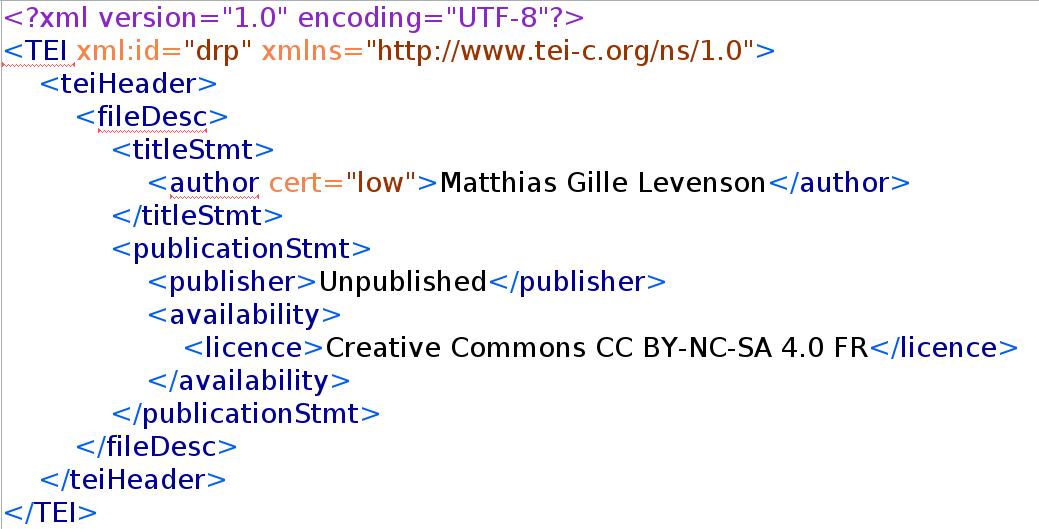
\includegraphics[height=.5\textheight]{img/element_attribute_text.png}
\caption{Ce document XML est \textbf{conforme} (mais la TEI est \textbf{invalide})}
\end{figure}
\end{center}
\end{frame}


\begin{frame}{Conformité}
\begin{itemize}
\item \textit{Pas} d'éléments qui se chevauchent
\end{itemize}
\begin{center}
\begin{figure}
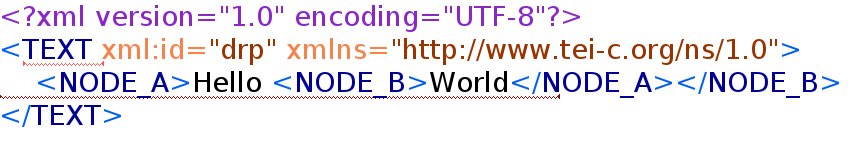
\includegraphics[width=.9\textwidth]{img/overlapping.png}
\caption{Ce document XML est non conforme}
\end{figure}
\end{center}
\end{frame}


\begin{frame}{Conformité}
\begin{itemize}
\item Certains éléments peuvent contenir d'autres éléments, mais ils peuvent aussi être vides
\end{itemize}
\begin{center}
\begin{figure}
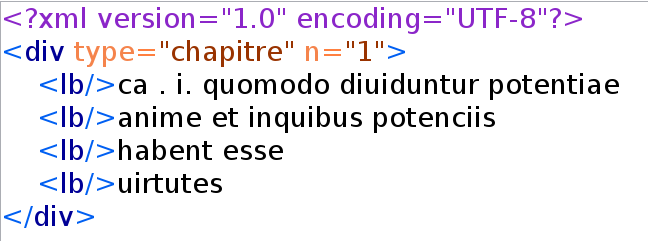
\includegraphics[width=.9\textwidth]{img/empty.png}
\caption{Ce document XML est conforme}
\end{figure}
\end{center}
\end{frame}



\begin{frame}{Conformité}
\begin{itemize}
\item Les valeurs d'attributs sont entre guillemets
\end{itemize}
\begin{center}
\begin{figure}
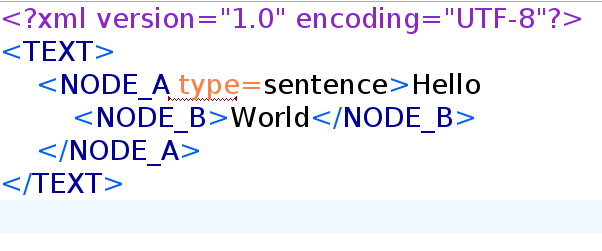
\includegraphics[height=.5\textheight]{img/attributes.png}
\caption{Ce document XML est non conforme}
\end{figure}
\end{center}
\end{frame}



\begin{frame}{Conforme? Non conforme?}
\begin{center}
\begin{figure}
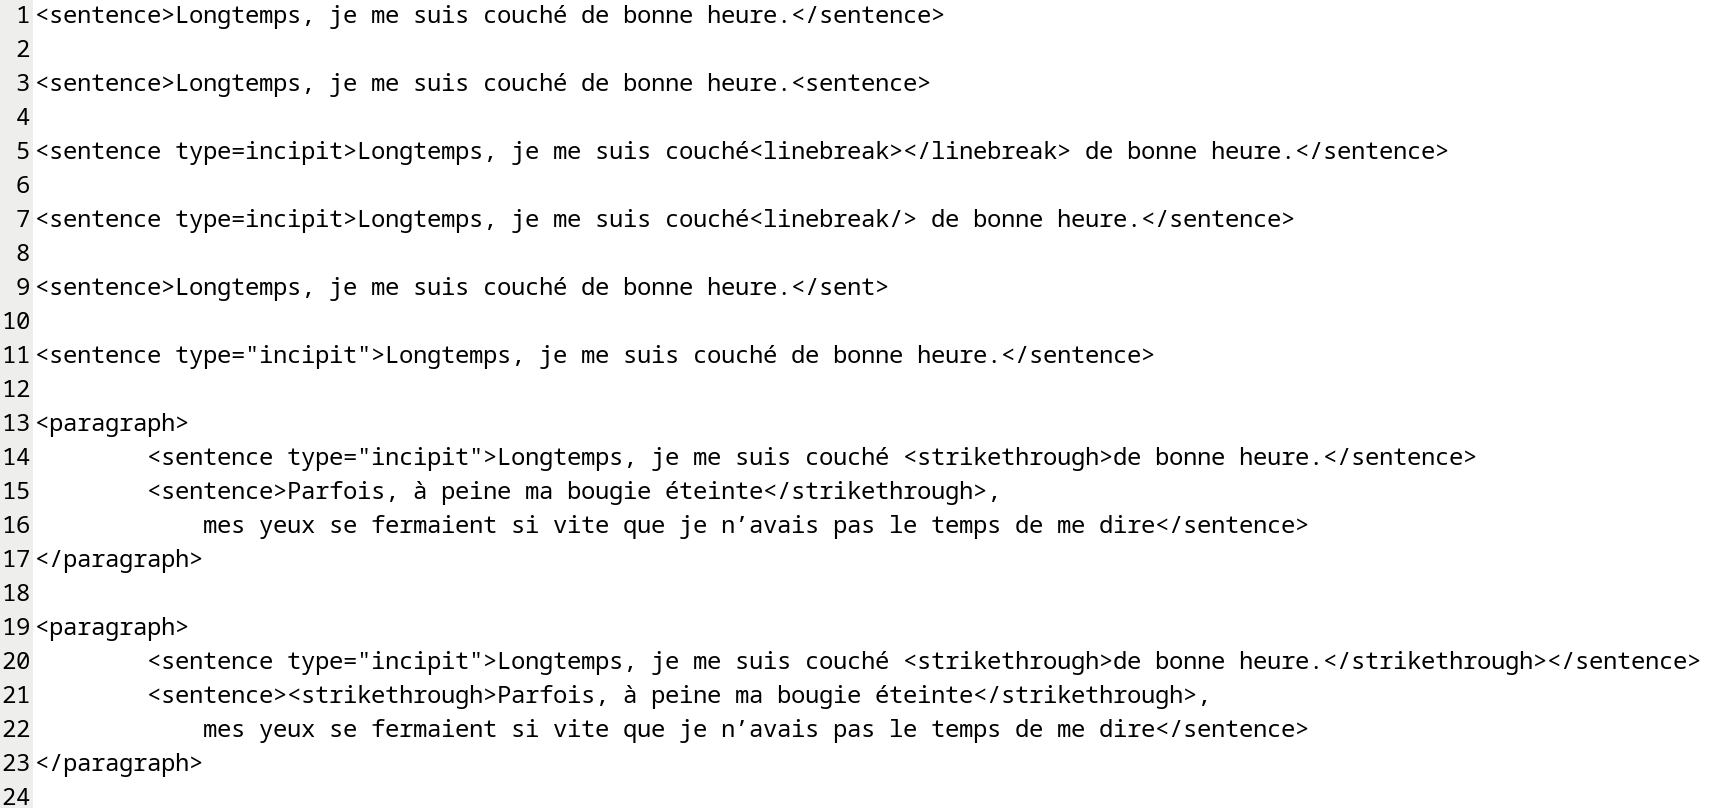
\includegraphics[height=.8\textheight]{img/conformant.png}
\end{figure}
\end{center}
\end{frame}


\subsection{Application. Corriger un XML mal structuré}

\begin{frame}{Oxygen}
\begin{itemize}
\item Oxygen XML editor est l'outil le plus utilisé, car il est développé en collaboration avec des utilisateur.ices de la TEI.
\item Il s'agit d'un outil propriétaire qui peut être remplacé par d'autres logiciels comme Jedit
\end{itemize}
\end{frame}

\begin{frame}{Raccourcis clavier dans Oxygen}
La touche ACTION correspond à CTRL sur Windows/Linux et POMME sur Mac.
\begin{itemize}
\item Créer un nouveau document: \texttt{ACTION + N}
\item Ouvrir un nouveau document: \texttt{ACTION + O}
\item Indenter (mettre en forme pour rendre lisible avec des sauts de lignes et des tabulations): \texttt{ACTION + SHIFT + P}
\item Commenter un fragment de document XML: \texttt{ACTION + SHIFT + ,}
\end{itemize}
\end{frame}


\begin{frame}{Application}
La touche ACTION correspond à CTRL sur Windows/Linux et POMME sur Mac.
\begin{itemize}
\item Ouvrez le document \texttt{session\_1\_introduction\_generale/exercices/exercice\_1.xml}
\item Indentez le document. Que se passe-t-il ?
\item Tâchez de réparer la structure afin d'avoir du XML conforme.
\item La lecture des messages d'erreur est souvent bien utile !
\end{itemize}
\end{frame}


\section{Qu'est-ce que la TEI?}

\subsection{Ce qu'est la TEI}
\begin{frame}{Qu'est-ce que la TEI?}
\begin{itemize}
\item Une communauté scientifique
\item Une \enquote{standard} et un ensemble de règles, les \textit{Guidelines}: \url{https://tei-c.org/release/doc/tei-p5-doc/en/html/}
\item Une façon de se représenter / modéliser \enquote{le} texte
\end{itemize}
\end{frame}


\subsection{Ce que n'est pas la TEI}


\begin{frame}{Ce que n'est pas la TEI}
\begin{itemize}
\item Un outil de visualisation des sources textuelles
\item Un outil de transformation des sources textuelles
\end{itemize}
\end{frame}


\begin{frame}{Ce qu'il vous faudra apprendre}
\begin{itemize}
\item Un langage de navigation dans le XML (XPath)
\item Un langage de transformation du XML pour la visualisation (XSLT, HTML)
\end{itemize}
\end{frame}


\subsection{Principes}
\begin{frame}{}
\begin{itemize}
\item Distinguer l'apparence et l'\enquote{essence} des objets textuels
\item Décrire cette \enquote{essence} selon un \textbf{consensus scientifique}
\end{itemize}
\begin{center}
\begin{figure}
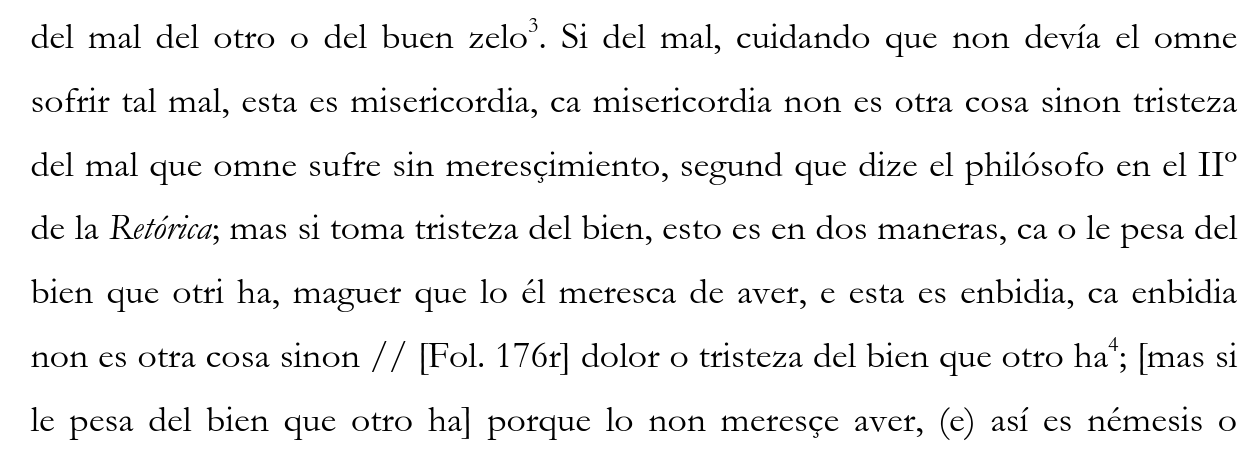
\includegraphics[width=.8\textwidth]{img/texte.png}
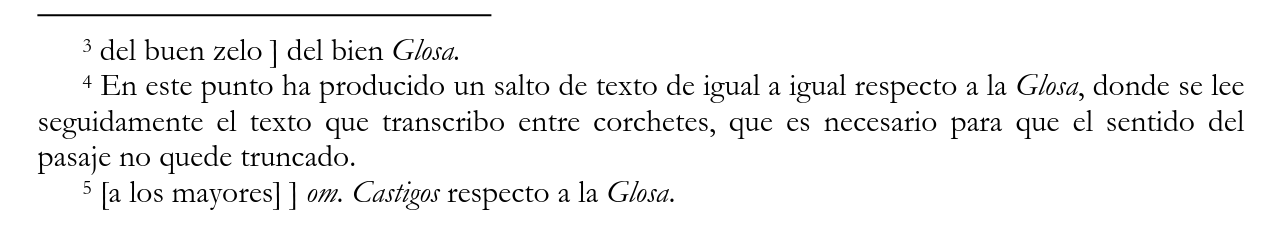
\includegraphics[width=.8\textwidth]{img/apparat.png}
\caption{Fragment d'une édition des \textit{Castigos de Sancho IV} \parencite{sanchez_VersionInterpoladaCastigos_2003}}
\end{figure}
\end{center}
\end{frame}

\begin{frame}
\begin{center}
\begin{figure}
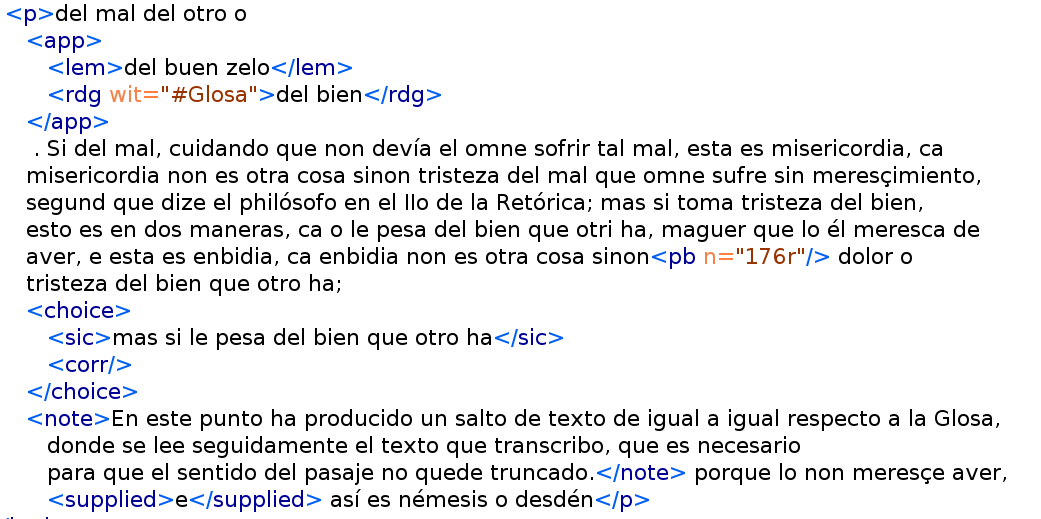
\includegraphics[width=.8\textwidth]{img/xml_structured.png}
\caption{Une représentation possible en XML-TEI}
\end{figure}
\end{center}
\end{frame}


\section{La TEI, pour quoi faire?}
\begin{frame}{La TEI, pour quoi faire?}
La TEI est le standard de fait pour le partage des données actuellement
\begin{itemize}
\item Pour décrire un objet textuel en utilisant l'expérience d'une communauté
\item Pour produire des données qui peuvent être \textbf{lues} par l'être humain et \textbf{traitées} par la machine
\item Pour faciliter l'échange de ces descriptions
\item Pour faciliter l'interopérabilité des données
\end{itemize}
\end{frame}


\begin{frame}[containsverbatim]{L'édition critique}
% Image TEI castillan / latin
\end{frame}



\begin{frame}[containsverbatim]{La critique génétique}
% Image TEI castillan / latin
\end{frame}

% https://stackoverflow.com/a/72696959
\begin{frame}[containsverbatim]{La collation automatisée}
\begin{minted}[breaklines, ,linenos,numbersep=3mm]{python}
for rdg in apps:
    if rdg.is_empty() and following_rdg.is_empty():
            create_node(witEnd)
\end{minted}
\end{frame}

\begin{frame}[containsverbatim]{L'alignement multilingue de sources vernaculaires médiévales}
% Image TEI castillan / latin
\end{frame}


\begin{frame}[containsverbatim]{L'alignement multilingue de sources vernaculaires médiévales}
% Table de concordance multilingue
\end{frame}

\section{Exemples utilisés au long de la formation}

\begin{frame}{}
\begin{itemize}
\item Un sonnet de Rimbaud
\item Une scène de \textit{L'avare} de Molière
\end{itemize}
\end{frame}


\begin{frame}{References}
\printbibliography
\end{frame}

\end{document}
